\documentclass{sig-alternate-05-2015}
\usepackage{float}
\usepackage{hyperref}


\begin{document}
% Copyright
%\setcopyright{acmcopyright}
% DOI
\doi{000000}

% ISBN
\isbn{000000}

\title{Access to Big Data in Bioinformatics}
% \subtitle{[Extended Abstract]}

\numberofauthors{1}
\author{
\alignauthor
Andrew van Rooyen\\
       \affaddr{University of Cape Town}\\
}

\date{30 August 2015}

\toappear{This paper and associated code is available at \url{https://github.com/wraithy/bigbinf}}

\maketitle
\begin{abstract}
\end{abstract}
% \keywords{Big Data; BioInformatics; Clouds}


\section{Background}

Data sets are a big part of bioinformatics, and have introduced many new challenges with the rise of next generation sequencing. Sequencing technologies like SOLiD provide much higher data output at a cheaper cost~\cite{shendure2008next}, which is good news for research, but troubling for data storage, transfer and access. In fact, the cost of storing a byte has been more expensive than sequencing a base pair since before 2010~\cite{baker2010next}.

This makes it difficult for researchers in different locations to manipulate and run processes on the data, because it will be stored in only one location. These files could be tens of gigabytes in size~\cite{deorowicz2011compression}, depending on context.

\subsection{Data storage}
Generally, once the sequencing machine has generated the raw information on each base pair, this data will be stored in a data warehouse. Storing this information for long periods of time requires the data to be structured efficiently in order to save space, and allow it to be transferred efficiently.
There has been a lot of work on how to structure this data. There are a plethora of file formats whose efficiency depends on the kind of data which needs to be stored. Two of the most popular formats are FASTQ, which stores aggregated reads along with the quality of each base pair~\cite{cock2010sanger}, and BAM, the binary, compressed version of the Sequence Alignment Map (SAM) format~\cite{SAMspec}.


\subsection{Data transfer}
When researchers require specific information for their projects, they need to be able to access the data warehouse and transfer whichever sequences they need. Luckily, these locations are often connected massive data pipes like National Research and Education Networks (NRENs). Unfortunately, standard protocols like FTP and SSH were never designed for use on high-throughput networks, and alternate protocols need to be used to avoid bottlenecking.

There are some proprietary transfer protocols which are widely used in practice. For example, the fasp protocol by the US based company AsperaSoft. Based on UDP, the protocol eliminates the latency issues seen with TCP, and provides bandwidth up to 10 gigabits per second to transfer data~\cite{beloslyudtsev2014aspera}.

\subsection{Alternate models}
There have been some attempts to do data processing remotely, and there has been an explorative push towards cloud solutions from Amazon, Google etc. Unfortunately, even though these cloud data centres have plenty of cheap storage, there are very significant drawbacks.

Because the sequencing happens in labs, researchers need to upload their raw data to the cloud data centres every time they run a new experiment. This leads back to the original problem, as researchers resort to mailing hard drives~\cite{baker2010next}.
There are also security, privacy and ethical concerns with outsourcing this processing power to other companies, as sequenced DNA data is often highly sensitive information~\cite{marx2013biology}.

\section{Design and Implementation}
\subsection{Design Aims} % (of the software)
The system will compare the following file transfer protocols to determine which is best for transferring bioinformatics data on an educational network: GridFTP, FTP, HPN-SSH and SCP.
These are the most popular protocols for file transfer in the field, perhaps with the exception of \textit{fasp} by AsperaSoft~\cite{beloslyudtsev2014aspera}, which is non-free. 

\subsection{Constraints}
In order to test the protocols in a relevant environment, the tests will be run between the University of Cape Town (UCT) and the University of the Western Cape (UWC). Both universities are connected to the South African National Research Network \cite{sanren} which runs at 10Gbps.\\\\
The `lite' version of GridFTP will be used. This means that authentication is done over ssh as opposed a previously-configured certificate authority. This makes no difference to the file transfer itself, but it prevents unnecessary configuration of the testbed which can be quite complex in the case of `full' GridFTP~\cite{gridftplite}.\\\\

\subsection{Approach}
% TODO: This is all over the place. Needs some structure.
Transfers using each of the 4 protocols will be run while the network traffic is logged.

The hosts will be virtual machines running at the South African National Bioinformatics Institute (UWC) and the Science DMZ (UCT). These locations were chosen because in both cases they are close to the SANReN link, and are on the outside of institutional firewalls. This means that throttling is avoided, and ensures a minimum speed of 1Gbps.
\begin{figure}[H]
	\label{fig:route}
	\centering
	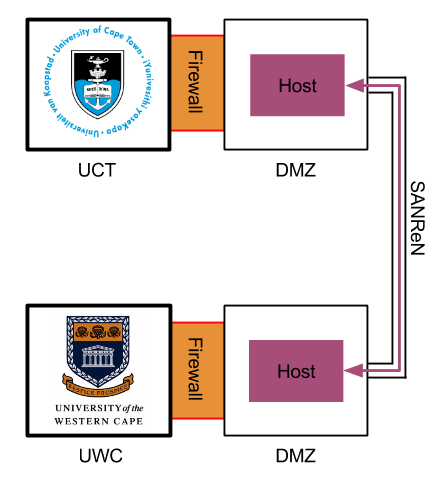
\includegraphics[width=0.4\textwidth]{img/route.png}
	\caption{The hosts in their environment.}
\end{figure}

The testing environment will be kept as stable as possible during tests, and multiple tests will be run at different times of the day.

A copy will be initiated from Host 1. A file from Host 2 will then be transferred to Host 1 using the particular protocol.
\begin{figure}[H]
	\label{fig:copy_example}
	\centering
	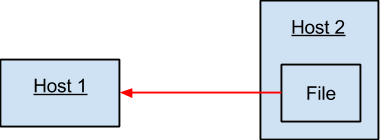
\includegraphics[width=0.4\textwidth]{img/basic_transfer_example.png}
	\caption{Host 1 copying a file.}
\end{figure}
Once the ideal protocol has been decided on, it will be made available as an endpoint to the microcloud system, so that users can retrieve their results in an optimal way.

\subsection{Evaluation}
%What is being measured/tested
The system will log packets on the network interface used for the transfer. This information can then be parsed by a suite of python tools to calculate metrics and display graphs.
This approach allows analysis of overhead (because \textit{all} transferred data is logged, rather than just the file size), speed (data/time), consistency, total time, and total size.

\subsection{Implementation}
A simple python script will be sufficient to run the transfers, as most of the work will be done by a subprocess for each specific protocol. The analysis will also be done using python as there are a vast number of analytical and visualisation tools available.\\\\
All testing will be done on an Ubuntu 14.04 system, with the following packages installed
\begin{itemize}
	\item python 2.7
	\item globus-gass-copy-progs 8.6
	\item globus-gridftp-server-progs 6.38
	\item tcpdump
	\item openssh-client
	\item openssh-server
	\item openssh-portable with the HPN patches, compiled from \url{https://github.com/rapier1/openssh-portable}
\end{itemize}
The testbed should work on any Unix system as long as python, tcpdump and the binaries for each protocol are installed correctly.
\\\\

\subsubsection{File transfer and logging}
The tests will be run with 3 files: A 6 byte file containing the word `hello', a 350MB video file and a 1GB video file. The formats of these files were not tailored to the specific domain of bioinformatics because all 4 protocols are agnostic of format, and treat everything as binary.

The `tcpdump' program (\url{www.tcpdump.org}) comes with most Unix systems. It watches a network interface (e.g.\ eth0) and logs information about packets which pass through. The program is run while the copy is in progress, and the output is filtered to include only packets sent between Host 1 and Host 2.
\begin{figure}[H]
	\label{fig:interface_example}
	\centering
	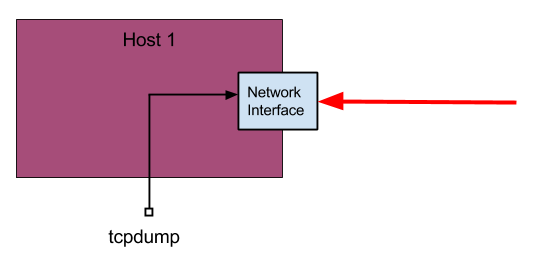
\includegraphics[width=0.5\textwidth]{img/if_example.png}
	\caption{The network interface capturing traffic.}
\end{figure}

Note that despite the name, tcpdump can also capture UDP packets, which is relevant for some of the protocols.

\subsubsection{Testbed}
The python script for running the file transfers has been written to accept
\begin{itemize}
	\item the name of the network interface
	\item the remote hostname (Host 2)
	\item the path of the file on Host 2
	\item a local path to copy the file to
\end{itemize}

It then resolves the IPs of each host, and for each protocol, runs a copy in isolation. It spawns a tcpdump subprocess, and lets it run for precisely as long as the copy runs. The tcpdump program is started with filters, so that only traffic between the two hosts is captured. It then saves the output in a file.\\\\
\begin{figure}[H]
	\label{fig:testbed_sequence}
	\centering
	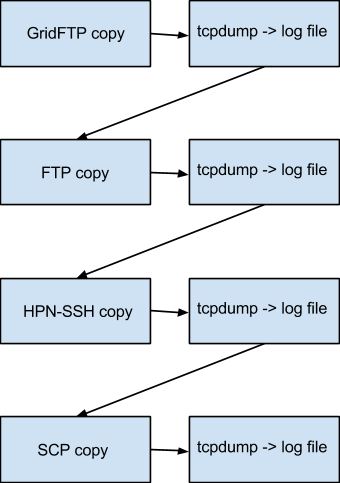
\includegraphics[height=0.5\textheight]{img/seq_example}
	\caption{The sequence of subprocesses called by the testbed.}
\end{figure}
Doing it this way allows for a much more controlled environment. Because the tcpdump is only capturing while the copy is running, no other packets will be included in the logs. Also, the copies are run programmatically and consecutively. Following copies are not started until both the tcpdump and protocol processes have been closed, and the log file has been written. This means that they are all run in an identical (within reason) environment, but at the same time do not interfere with each other.

This test process is run multiple times for statistical reasons, generating multiple log files.

\subsubsection{Analysis of dumps}
A separate python file reads in the log files and parses them. Operations can then be run by looking at the time of each packet, and the size of its payload. 

This data can then be aggregated over multiple log files, and graphed using the matplotlib python library.\\\\
More info is needed here, and will be filled in once I have completed the analysis scripts.

\bibliographystyle{ACM-Reference-Format-Journals}
\bibliography{ref} 


\end{document}
